% introduction.tex
% contains the text for the Introduction section of the manuscript
% paper-draft-tex/templates/src

\section{Introduction \label{sec:introduction}}
	In~\cite{ACleverResearcher2023}, they show that for researchers is crucial to focus on research findings.
	\reffig{fig:cool-images} shows a relaxed cat. 
	Note that the first author in~\cite{ACleverResearcher2023} loves cats.
	
	\begin{figure}[H]
		\centering
		% You might want to adjust the image, since it does not have axes, labels or fonts
		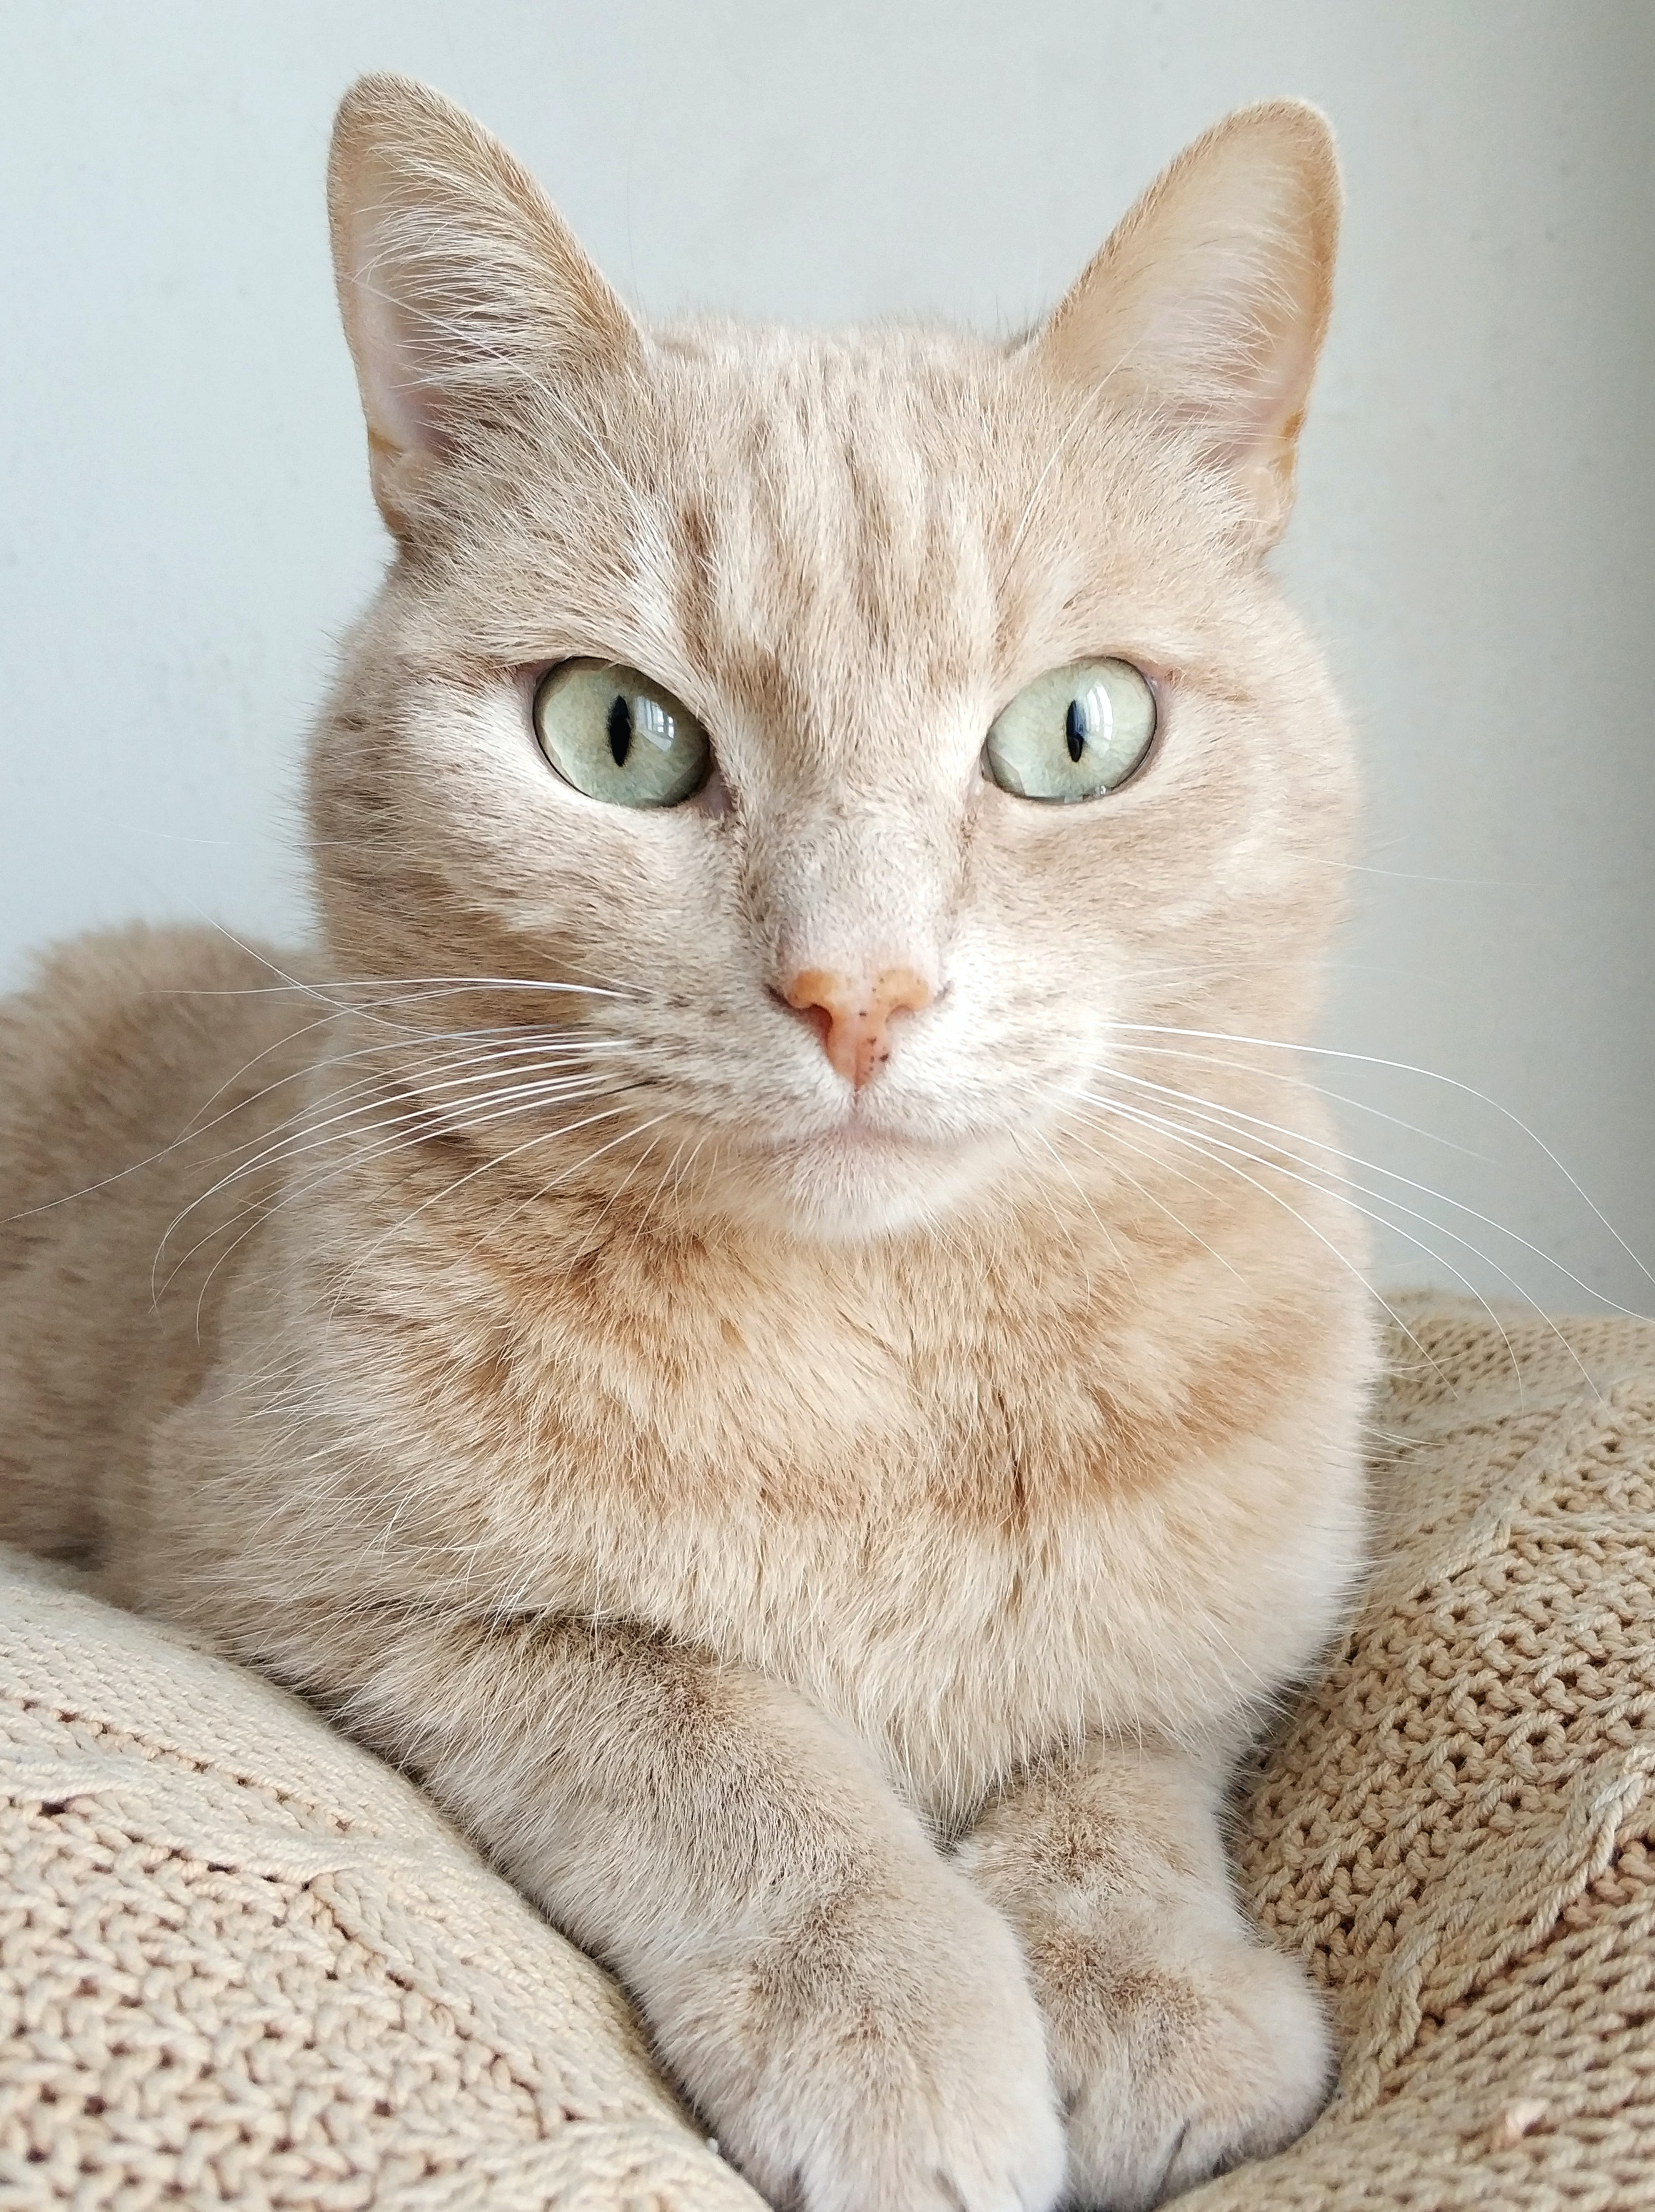
\includegraphics[height=.5\textwidth]{fig/nice-cat.jpg}
		\caption{
			A relaxed cat picture, saved in JPG format. \href{https://www.pexels.com/photo/orange-tabby-cat-on-brown-knitted-textile-982300/}{Source}.
			\label{fig:cool-images}
		}
	\end{figure}
	
